
%(BEGIN_QUESTION)
% Copyright 2015, Tony R. Kuphaldt, released under the Creative Commons Attribution License (v 1.0)
% This means you may do almost anything with this work of mine, so long as you give me proper credit

\noindent
{\bf Lab Exercise}

\vskip 5pt

Your primary task is to independently (i.e. no assistance from team members or other classmates) tune multiple control loops, documenting the process open-loop response as well as the process closed-loop responses to both setpoint and load changes.  This documentation must be in the form of computer screen captures, showing the graphic trends of the process as it responds to open-loop and closed-loop tests.  You must do your own loop testing and tuning, the consequence of plagiarism being a failing grade for the course.

Two of the processes you will tune must be {\it real}, working processes.  The last process may be simulated, or it may be another real process with different characteristics than the first two.  All tuning objectives are ``mastery'' -- they must be demonstrated to instructor satisfaction for completion, with no penalty for multiple attempts.

\vskip 10pt

\underbar{Process tuning table:}

% No blank lines allowed between lines of an \halign structure!
% I use comments (%) instead, so that TeX doesn't choke.

$$\vbox{\offinterlineskip
\halign{\strut
\vrule \quad\hfil # \ \hfil & 
\vrule \quad\hfil # \ \hfil & 
\vrule \quad\hfil # \ \hfil & 
\vrule \quad\hfil # \ \hfil \vrule \cr
\noalign{\hrule}
%
% First row
{\bf Performance objective} & {\bf Real \#1} & {\bf Real \#2} & {\bf Real \#3 or Simulated} \cr
%
\noalign{\hrule}
%
% Another row
Description of process &  &  &  \cr
%
\noalign{\hrule}
%
% Another row
Self-reg. {\it vs.} Integ. {\it vs.} Runaway? &  &  &  \cr
%
\noalign{\hrule}
%
% Another row
Measurement of dead time (sec) &  &  &  \cr
%
\noalign{\hrule}
%
% Another row
Measurement of time constant (sec) &  &  &  \cr
%
\noalign{\hrule}
%
% Another row
Measurement of valve stiction (\%) &  &  &  \cr
%
\noalign{\hrule}
%
% Another row
P value after tuning ($K_p$) &  &  &  \cr
%
\noalign{\hrule}
%
% Another row
I value after tuning ($K_i$ or $\tau_i$) &  &  &  \cr
%
\noalign{\hrule}
%
% Another row
D value after tuning ($K_d$ or $\tau_d$) &  &  &  \cr
%
\noalign{\hrule}
%
% Another row
Robust response to SP change? &  &  &  \cr
%
\noalign{\hrule}
%
% Another row
Robust response to load change? &  &  &  \cr
%
\noalign{\hrule}
%
% Another row
{\it Instructor initials} &  &  &  \cr
%
\noalign{\hrule}
%
% Another row
Decommission and lab clean-up &  & -- -- -- -- & -- -- -- -- \cr
%
\noalign{\hrule}
%
% Another row
Team tool locker inspection &  & -- -- -- -- & -- -- -- -- \cr
%
\noalign{\hrule}
} % End of \halign 
}$$ % End of \vbox

In addition to process tuning, you must also troubleshoot a control system and answer lab questions, the same as in regular team-based lab exercises.  A crucial different is that none of the objectives in this entire lab exercise are team-based; rather, all are individual. 

\vskip 10pt

\underbar{Objective completion table:}

% No blank lines allowed between lines of an \halign structure!
% I use comments (%) instead, so that TeX doesn't choke.

$$\vbox{\offinterlineskip
\halign{\strut
\vrule \quad\hfil # \ \hfil & 
\vrule \quad\hfil # \ \hfil \vrule \cr
\noalign{\hrule}
%
% First row
{\bf Performance objective} & pass/score \cr
%
\noalign{\hrule}
%
% Another row
Troubleshooting &   \cr
%
\noalign{\hrule}
%
% Another row
Lab question: Instrument connections &  \cr
%
\noalign{\hrule}
%
% Another row
Lab question: Tuning &  \cr
%
\noalign{\hrule}
%
% Another row
Lab question: Mental math &  \cr
%
\noalign{\hrule}
%
% Another row
Lab question: Diagnostics &  \cr
%
\noalign{\hrule}
} % End of \halign 
}$$ % End of \vbox

\vskip 10pt

The only ``proportional'' scoring in this activity are the lab questions, which are answered by each student individually.  A listing of potential lab questions are shown at the end of this worksheet question.  The lab questions are intended to guide your labwork as much as they are intended to measure your comprehension, and as such the instructor may ask these questions of your team day by day, rather than all at once (on a single day).

When everyone is finished tuning and troubleshooting loops, the last step is to decommission all the working systems as per usual procedure.

\vskip 10pt

{\bf Note: this lab worksheet is your only record of the instructor's validation (signed initials).  Do not lose it, and do not lose your screen-captures of the process responses either!}





\vfil \eject

\noindent
{\bf Lab Exercise -- how to capture ``screen-shots'' on a PC}

\vskip 5pt

An essential part of this lab exercise is capturing graphical trend data from the screen of a personal computer, either running control software (e.g. Emerson DeltaV Operate) or data acquisition software used to monitor process data (e.g. WinDAQ, LabVIEW).  Fortunately, this is really easy to do on any personal computer. 

When you have the screen of the computer displaying what you wish to capture, simply press the ``Print Screen'' key on your keyboard.  This key is usually located to the right of the ``Function'' key row at the top (on a standard desktop keyboard layout -- laptop keyboards are famous for locating seldom-used keys like this in random places).  Pressing the ``Print Screen'' key tells the computer's operating system to copy the entire screen image into a buffer for pasting into any graphics-manipulation or word-processing program you desire.

A utility standard on every Windows operating system is {\it Paint}: a bitmap image creation and manipulation program.  Paint is simple to the point of being crude, but it works just fine for this purpose.  After starting Paint, simply ``Paste'' the captured screen-shot image and save it under any filename you wish.  I strongly recommend using a filename that is unique to you (e.g. {\tt John\_Doe\_process1\_trend2.bmp}).  Remember that you will be capturing multiple screen-shots in this lab exercise, and will need to save every one for presentation to the instructor.  

You may also use Paint (or even a more sophisticated image-manipulation program such as {\it Photoshop} or {\it Gimp}) to add text annotations to your screen-shot images.  For example, some students like to add arrows and lines showing where they measured process gain, or arrows pointing to problems in the trend such as where the control valve sticks.

\vskip 10pt

{\bf Common mistakes:}

\begin{itemize}
\item{} Forgetting to move screenshot files to personal drive, leaving them on the hard drive of the school computer where they may be deleted by other students
\end{itemize}






\vfil \eject

\noindent
{\bf Lab Exercise -- open-loop testing}

\vskip 5pt

Before you can begin to successfully tune a PID-controlled process, you must first understand the characteristics of that process.  A very good way to do this is by performing an {\it open-loop} test: placing the PID controller in manual mode and changing the output value (5\% or so is usually a good amount for the first test) to see what effect this has on the process variable over time.  The PV's response to this ``step-change'' in output can not only reveal the basic characteristics of the process (i.e. self-regulating, integrating, runaway, lag time magnitude, lag order(s), dead time magnitude) but also certain instrument problems (valve stiction, transmitter filtering, etc.).

You should perform several open-loop step-changes to probe the process characteristics: a few in the same direction, then the rest in the other direction.  An analysis of the PV responses following multiple output step-changes will reveal two important characteristics of the process:

\begin{itemize}
\item{} How consistent the process gain is
\item{} Whether the valve has significant hysteresis or stiction (compare opening versus closing)
\end{itemize}

$$\includegraphics[width=15.5cm]{i01675x02.eps}$$

\vskip 10pt

\filbreak

Valve stiction may be determined by making alternating (up and down) step-changes in manual mode in progressively smaller intervals, noting the largest of those step-changes resulting in no measureable PV change.  The following illustration shows this test applied to a fast, self-regulating process:

$$\includegraphics[width=15.5cm]{i01675x03.eps}$$

\vskip 10pt

{\bf Common mistakes:}

\begin{itemize}
\item{} Trying to probe the process characteristics with the controller in {\it automatic} mode rather than {\it manual} mode
\item{} Making output step-changes that are too large (resulting in PV excursions)
\item{} Not making enough step-changes to fully test process gain consistency or valve stiction
\end{itemize}







\vfil \eject

\noindent
{\bf Lab Exercise -- decide on a tuning strategy}

\vskip 5pt

After you have determined the characteristics of the process and corrected any instrument problems such as transmitter filtering or valve stiction, your next step is to determine how you will tune the PID controller.  Several algorithmic procedures exist, including two methods proposed by Ziegler and Nichols in their 1942 paper, and several more modern methods.  You are free to use whatever tuning method you would like to try, so long as you document the data supporting your tuning decisions (i.e. process characteristics) and also document the trend data showing improvement in process stability as you use your understanding of PID control to fine-tune each process.

Truth be told, many working professionals use algorithmic methods such as Ziegler-Nichols because they really don't understand how PID works, or is supposed to be applied to a real process.  The goal of this lab exercise is to give you plenty of opportunity to try your hand at PID tuning, and to improve upon simple step-by-step methods such as Ziegler-Nichols.  With practice, you will find it possible to make dramatic improvements over ``canned'' PID tuning methods simply by understanding the characteristics of the process and choosing control actions appropriate for those characteristics.

\vskip 10pt

The following table shows several PV responses following a single controller output step-change in manual mode, with suggesting heuristic tuning strategies for each:

$$\includegraphics[width=15.5cm]{i01675x01.eps}$$

Remember that the presence of certain other characteristics in significant amounts (e.g. PV noise, dead time, etc.) also impacts how one should tune a controller. 

\vskip 10pt

{\bf Common mistakes:}

\begin{itemize}
\item{} Making tuning parameter changes that are too large without considering the ill effects those changes might have (e.g. increasing gain by a factor of 10)
\item{} Attempting to ``de-tune'' process or instrument problems that should be repaired (transmitter filtering, valve stiction, etc.)
\end{itemize}









\vfil \eject

\noindent
{\bf Lab Exercise -- robust PID response}

\vskip 5pt

In this exercise you will be asked to demonstrate ``robust'' loop response to both setpoint changes and load changes, which naturally demands a definition for ``robust'' response.  In this context, robust PID response is such that the PV is brought to setpoint as fast as possible, with as little over/undershoot as possible, and absolutely no ``porpoising'' (oscillations prior to reaching setpoint).

\vskip 10pt

A controller that is tuned too ``fast'' will take little time reaching setpoint, but it will do so at the expense of overshooting or undershooting the setpoint value before settling in to the setpoint value.  A controller that is tuned too ``slow'' will not over- or under-shoot setpoint, but will exhibit extended periods of time where the PV is approaching setpoint yet the output value is nowhere near saturation (i.e. the controller is not ``trying'' as hard as it can).

\vskip 10pt

When testing for robust response to load changes, you should introduce load changes in a manner similar to how you introduce setpoint changes: change the load {\it and leave the load in that new state long enough to watch the controller compensate for it.}  A very common error students make when introducing load changes is to do so very briefly, so briefly in fact that the controller never gets a chance to correct for the new load condition.  What you see in such a case is the PV changing due to the load change, and then returning back to setpoint {\it only because the load returned to its previous value, not because the controller actually did anything to make PV return to setpoint!}  So remember, when you introduce load changes, do so the same way you introduce setpoint changes: change the load condition and leave it in that new state, then watch the controller's response to see how quickly the PV returns to the setpoint value, whether there is under- or over-shooting of the setpoint, and/or whether any porpoising occurs.

\vskip 10pt

You will notice that ideal tuning for response to setpoint changes is often different from ideal tuning for response to load changes.  One reason for this is that setpoint changes typically occur more suddenly than load changes.  Another reason is that load changes tend to alter the processes' equilibrium point (i.e. the FCE value necessary to maintain the setpoint) more than setpoint changes.  If you notice a great different between these two responses, you may wish to set the PID algorithm to one where more of the PID equation responds only to changes in {\it PV} and not to changes in {\it error}.

\vskip 10pt

If your controller ``porpoises'' at all, it is detrimental to process control.  ``Porposing'' occurs when either the controller's proportional action or derivative action is too aggressive, causing the controller to over-correct during the PV's approach to setpoint.  Integral is incapable of causing porpoising, because integral action cannot reverse direction unless and until the error changes sign (i.e. until PV crosses setpoint), and porpoising is defined as oscillations occuring {\it prior} to setpoint.  Perhaps the best tool for determining whether excessive gain or excessive derivative action is causing porpoising is to examine the {\it phase shift} between PV and Output during the porpoising period: little or no phase shift reveals excessive P action, while nearly 90$^{o}$ phase shift reveals excessive D action.


\vfil

{\bf Common mistakes:}

\begin{itemize}
\item{} Not properly diagnosing field instrument problems (e.g. sticky valves, over-damped transmitters) prior to tuning.  {\it Pay close attention to your open-loop tests prior to any PID tuning parameter adjustments!!!}
\item{} Relying too much on proportional action (gain) to control fast-acting, self-regulating processes.
\item{} Introducing transient load changes that don't persist long enough to test the controller's ability to correct (i.e. to bring the PV back to SP with different load conditions).
\end{itemize}











\vfil \eject

\noindent
{\bf Lab Exercise -- troubleshooting}

\vskip 5pt

The most challenging aspect of this lab exercise is {\it troubleshooting}, where you demonstrate your ability to logically isolate a problem in the system.  All troubleshooting is done on an individual basis (no team credit!), and must be done {\it on a system you did not help build}, so that you must rely on loop diagrams to find your way around the system instead of from your own memory of building it.

Each student is given a limited amount of time to identify both the general location and nature of the fault, logically justifying all diagnostic steps taken.  All troubleshooting activities will take place under direct instructor supervision to ensure students are working independently and efficiently. 

Failure to correctly identify both the general location and nature of the fault within the allotted time, and/or failing to demonstrate rational diagnostic procedure to the supervising instructor will disqualify the effort, in which case the student must re-try with a different fault.  Multiple re-tries are permitted with no reduction in grade.

A standard multimeter is the only test equipment allowed during the time limit.  No diagnostic circuit breaks are allowed except by instructor permission, and then only after correctly explaining what trouble this could cause in a real system.  

The instructor will review each troubleshooting effort after completion, highlighting good and bad points for the purpose of learning.  Troubleshooting is a skill born of practice and failure, so do not be disappointed in yourself if you must make multiple attempts to pass!  One of the important life-lessons embedded in this activity is how to deal with failure, because it {\it will} eventually happen to you on the job!  There is no dishonor in failing to properly diagnose a fault after doing your level best.  The only dishonor is in taking shortcuts or in giving up.

\vskip 10pt

\filbreak

Recall that every feedback control loop consists of four basic elements: an element that {\it senses} the process variable (e.g. primary sensing element, transmitter), an element that {\it decides} what how to regulate this process variable (e.g. a PID controller), an element that {\it influences} the process variable (e.g. a control valve, motor drive, or some other final control device), and finally the process itself which {\it reacts} to the final control device's actions:

$$ \includegraphics[width=15.5cm]{i01675x05.eps}$$

\noindent
You can check each element of your feedback control loop by comparing its input with its output to see if each element is doing what it should:

\begin{itemize}
\item{$(1)$} \underbar{\bf Decision-making:} Carefully examine the controller faceplate, looking at the values of PV, SP, and Output.  Is the controller taking appropriate action to force PV equal to SP?  In other words, is the Output signal at a value you would expect if the controller were functioning properly to regulate the process variable at setpoint?  If so, then the controller's action and tuning are most likely not at fault.  If not, then the problem definitely lies with the controller.
\item{$(2)$} \underbar{\bf Sensing:} Compare the controller's displayed value for PV with the actual process variable value as indicated by local gauges, by feel, or by any other means of detection.  If there is good correspondence between the controller's PV display and the real process variable, then there probably isn't anything wrong with the measurement portion of the control loop (e.g. transmitter, impulse lines, PV signal wiring, analog input of controller, etc.).  If the displayed PV disagrees with the actual process variable value, then something is definitely wrong here.
\item{$(3)$} \underbar{\bf Influencing:} Compare the controller's displayed value for Output with the actual status of the final control element.  If there is good correspondence between the controller's Output display and the FCE's status, then there probably isn't anything wrong with the output portion of the control loop (e.g. FCE, output signal wiring, analog output of controller, etc.).  If the controller Output value differs from the FCE's state, then something is definitely wrong here.
\item{$(3)$} \underbar{\bf Reacting:} Compare the process variable value with the final control element's state.  Is the process doing what you would expect it to?  If so, the problem is most likely not within the process (e.g. manual valves, relief valves, pumps, compressors, motors, and other process equipment).  If, however, the process is not reacting the way you would expect it to given the final control element's state, then something is definitely awry with the process itself.
\end{itemize}





\vskip 10pt

\filbreak

{\bf Common mistakes:}

\begin{itemize}
\item{} Neglecting to take measurements with your multimeter.
\item{} Neglecting to check other measurements in the system (e.g. pressure gauge readings).
\item{} Incorrectly interpreting the loop diagram (e.g. thinking you're at the wrong place in the system when taking measurements).
\item{} Incorrect multimeter usage (e.g. AC rather than DC, wrong range, wrong test lead placement).  This is especially true when a student comes to lab unprepared and must borrow someone else's meter that is different from theirs!
\end{itemize}

\vskip 10pt

{\bf Remember that the purpose of the troubleshooting exercise is to foster and assess your ability to intelligently diagnose a complex system.  Finding the fault by luck, or by trial-and-error inspection, is not a successful demonstration of skill.  The only thing that counts as competence is your demonstrated ability to logically analyze and isolate the problem, correctly explaining all your steps!}

\vskip 10pt

{\bf Troubleshooting takes a lot of lab time, usually at least two 3-hour lab sessions for everyone in a full class to successfully pass.  Be sure your team budgets for this amount of time as you plan your work, and also be sure to take advantage of your freedom to observe others as they troubleshoot, to better learn this art.}






\vfil \eject

\noindent
{\bf Lab questions}

\vskip 5pt

\begin{itemize}
\item{} {\bf Instrument connections}
\item{} Determine correct wire connections between instruments to create a working 4-20 mA loop circuit, based on diagrams of instruments with terminals labeled
\item{} Correctly determine all electrical sources and loads, as well as all voltage polarities and current directions in a 4-20 mA loop circuit, based on diagrams of instruments with terminals labeled
\end{itemize}

\filbreak

\begin{itemize}
\item{} {\bf Tuning techniques}
\item{} Describe the open-loop method of tuning as designed by Ziegler and Nichols
\item{} Describe the closed-loop (``ultimate'') method of tuning as designed by Ziegler and Nichols
\item{} Identify process types that respond well to aggressive proportional action
\item{} Identify process types that respond poorly to aggressive proportional action
\item{} Identify process types that respond well to aggressive integral (reset) action
\item{} Identify process types that respond poorly to aggressive integral (reset) action
\item{} Identify process types that respond well to aggressive derivative (rate) action
\item{} Identify process types that respond poorly to aggressive derivative (rate) action
\end{itemize}

\filbreak

\begin{itemize}
\item{} {\bf Mental math} (no calculator allowed!)
\item{} Convert a proportional band value into a gain value
\item{} Convert a gain value into a proportional band value
\item{} Convert a repeats/(minute or second) integral value into a (minutes or seconds)/repeat integral value, or vice-versa
\item{} Convert between different pressure units, without relying on the use of a reference for conversion factors (i.e. you must commit the major conversion factors to memory)
\item{} Calculate the pneumatic pressure in a 3-15 PSI range corresponding to $x$ percent.
\item{} Calculate the electrical current in a 4-20 mA range corresponding to $x$ percent.
\item{} Calculate the electrical voltage in a 1-5 volt range corresponding to $x$ percent.
\item{} Calculate the percentage value of a pneumatic pressure signal $x$ PSI in a 3-15 PSI range.
\item{} Calculate the percentage value of an electrical current signal $x$ mA in a 4-20 mA range.
\item{} Calculate the percentage value of an electrical voltage signal $x$ volts in a 1-5 volt range.
\end{itemize}

\filbreak

\begin{itemize}
\item{} {\bf Diagnostics}
\item{} Explain how to distinguish an ``open'' cable fault from a ``shorted'' cable fault using only a voltmeter (no current or resistance measurement, but assuming you are able to break the circuit to perform the test)
\item{} Determine whether or not a given diagnostic test will provide useful information, given a set of symptoms exhibited by a failed system
\item{} Identify at least two plausible faults given the results of a diagnostic test and a set of symptoms exhibited by a failed system
\item{} Propose a diagnostic test for troubleshooting a failed system and then explain the meanings of two different test results
\end{itemize}



\vfil \eject

\noindent
{\bf Lab Exercise -- decommissioning}

\vskip 5pt

The final step of this lab exercise is to decommission your team's entire system and re-stock certain components back to their proper storage locations, the purpose of which being to prepare the lab for the next lab exercise.  Remove your system documentation (e.g. loop diagram) from the common holding area, either discarding it or keeping it for your own records.  Also, remove instrument tag labels (e.g. FT-101) from instruments and from cables.

\vskip 10pt

\indent
{\bf Leave the following components in place, mounted on the racks:}

\begin{itemize}
\item{} Large control valves and positioners
\item{} I/P transducers
\item{} Large electric motors
\item{} Large variable-frequency drive (VFD) units
\item{} Cables inside conduit interconnecting junction boxes together
\item{} Pipe and tube fittings (do not unscrew pipe threads)
\item{} Supply air pressure regulators
\end{itemize}

\vskip 10pt

\indent
{\bf Return the following components to their proper storage locations:}

\begin{itemize}
\item{} Sensing elements (e.g. thermocouples, pH probes, etc.)
\item{} Process transmitters
\item{} ``Jumper'' cables used to connect terminal blocks within a single junction box
\item{} Plastic tubing and tube fittings (disconnect compression-style tube fittings)
\item{} Power cables and extension cords
\item{} Adjustment (loading station) air pressure regulators
\end{itemize}

\vskip 10pt

Finally, you shall return any control system components to their original (factory default) configurations.  This includes controller PID settings, function block programs, input signal ranges, etc.


\underbar{file i01675}
%(END_QUESTION)





%(BEGIN_ANSWER)


%(END_ANSWER)





%(BEGIN_NOTES)

{\bf Troubleshooting fault ideas:}

\begin{itemize}
\item{} Connect instrument tubes to wrong port (construction fault)
\item{} Replace I/P restrictor with pre-faulted (plugged) unit (high output fault)
\item{} Replace I/P relay with pre-faulted unit (low or high output fault)
\item{} Turn supply air pressure down well below 15 PSI (low output fault)
\item{} Strip wire at terminal, then insert insulated wire end under terminal and tighten (open wire fault)
\item{} Cut signal cable somewhere in mid-conduit (open wire fault)
\item{} Push a thumbtack through the cable somewhere in mid-conduit (shorted wire fault)
\item{} Wire instrument cable conductors backward (construction fault)
\item{} Plug tube connections using portion of foam earplug stuffed into tube fitting (slow response fault)
\item{} Configure transmitter for excessive damping (slow response fault)
\item{} Configure indicator/controller for excessive damping (slow response fault)
\item{} Mis-configure linear/sq.root characterization of transmitter and/or indicator/controller (nonlinearity fault)
\item{} Miscalibrate transmitter and/or indicator/controller (inaccuracy fault)
\item{} Connect 2.2 k resistor in parallel with 4-20 mA transmitter to simulate partial short in wiring (inaccuracy fault)
\item{} Exchange 250 ohm resistor for a different resistor that looks the same but has the wrong value (inaccuracy fault) 
\item{} Reverse action of controller/positioner/transmitter (wrong response fault)
\item{} Close air supply block valve and leave safety tag hanging on it (operator/technician error)
\item{} Give students wrong loop diagram (documentation fault)
\end{itemize}














\vfil \eject

\noindent
{\bf Lab questions}

\vskip 20pt

\item{$(1)$} Give step-by-step instructions for measuring the amount of {\it dead time} in a control loop.

\vskip 20pt

\item{$(2)$} Consider the water level control system shown below, for a flare gas water seal drum.  Assuming the water level signal (PV) is noise-free, that load changes are small and infrequent, that we don't care how suddenly the control valve may move as it regulates water level, and that the process itself exhibits an {\it integrating} characteristic, predict whether or not the level controller will regulate water level well with:
\begin{itemize}

\item{} Aggressive integral (I) control action: {\it Yes} or {\it No}?

\vskip 20pt

\item{$(3)$} Convert an integral controller setting of 0.5 minutes per repeat into {\it repeats per second}.

\vskip 20pt

\item{$(4)$} Suppose the water seal drum level control system shown below has a problem: LG-5 registers a steady water level of 30\% while LIC-21 registers a steady water level of 50\%.  Local indicator LI-21 also registers a steady water level of 50\%.  The setpoint of LIC-21 is at 50\% and the controller has been in automatic mode the whole time.  Identify one possible fault, as well as one impossible fault, with regard to these symptoms.  Be specific in your identification: both the location (which component) and nature (e.g. open, shorted, plugged) of each fault.

$$\includegraphics[width=15.5cm]{i01675x04.eps}$$ 

%INDEX% Lab exercise, control loop tuning

%(END_NOTES)


